\chapter{Electromagnetic Worldlines - Numerical Methods and Results}
\label{ch:numerical}
\begin{enumerate}
\item Need to develop methods that can easily generalize to more complicated geometries.
\item Even if using them to solve known problems.
\item In same fashion path integral relies on chaining together correct short-time propagator, we 
  are effectively using planar results at each step, under the assumption that the geometry
    is well-described locally by a single nearby plane.  
\item Need to study convergence effects carefully.  
\end{enumerate}

\section{Numerical Methods}



\subsection{Monte-Carlo sampling}

\begin{enumerate}
\item Need average over ensemble of paths.
\item For a Dirichlet scalar, can determine the set of times when integral is non-zero and 
  integrate over that.  In this case, the loop potential is either zero or one, with no variation.
  Thus it is more straightforward to integrate over space/loop-time.  
\item For computationally expensive loops, it makes sense to sample only a single position, time.
  Explore a larger ensemble in the same computational time.
  \item Rely on importance sampling to determine most important regions of $x_0$, $T$ to sample from.
  \item For time: For TE loops, integrand is zero before first touching time.  
    So use $P(\cT,\cT_0) = 2\cT_0^2\theta(\cT-\cT_0)/\cT^3$.
    TM loops turn on more softly, due to potential terms (which take into account possible sub-paths
    that touch the surface).
  \item Birth-death method effectively examines a larger ensemble of loops.
    For two-bodies, it is possible to spawn new loops while close to only a single surface,
    that might touch the other surface.  Thus the first-touching time for the parent loop
    is a poor estimate.  Simplest to use an ensemble average estimate for time:
    $P(\cT,d_0) = \exp(-2d_0^2/\cT)/\cT^3$, where exponential factor is the first touching
    time.  
  \item For spatial integrals, sample from uniform distribution within a radius that bounds all objects.
    Then sample from a power-law outside that, where estimate follows from first-touching time.
    May be possible to optimize, but captures important features without biasing
  \item Frequency integrals: Can execute in parallel (like picking different $chi$).
\end{enumerate}


\subsection{Sampling Times}

For a given discrete Brownian Bridge $\vect{x}_j$, there are a couple ways to sample the times.

\subsubsection{First-touching time}

The simplest method which applies to TE/sojourn integrands is to find the first-touching time, $T_0$
when the renormalized integrand first takes on a non-zero value.  After that point $T_0$, the
integrand will slowly increase due to the increased sojourn value as more point pass into the 
surfaces.  However, there is an additional $1/T^{1+D/2}$ factor which damps these contributions out.

This suggests sampling from a probability distribution 
\begin{equation}
  P(T;T_0,m)= \frac{(m-1) T_0^{m-1}}{T^m}\Theta(T-T_0),
\end{equation}
where $m>1$ and $T_0>0$.  This requires being able to estimate the value of $T_0$.  For the example
of paths starting between parallel planes $T_0=\text{min}[\left(\frac{-d_1-x_0}{B_-}\right)^2,
\left(\frac{d_2-x_0}{B_+}\right)^2]$ where $d_1<x_0<d_2$.    

In order to sample from this distribution, we must invert 
\begin{equation}
  r=(m-1) T_0^{m-1}\int_{T_0}^T dt\, t^{-m}
\end{equation}
where $r\in [0,1]$ is a uniform random number and $T$ is the desired deviate.    
This can be straightforwardly inverted 
\begin{align}
  r&=(m-1) T_0^{m-1}\frac{1}{m-1}\left(\frac{1}{T_0^{m-1}}-\frac{1}{T^{m-1}}\right)\\
%  \left(\frac{T_0}{T}\right)^{m-1}&= (1-r)\\
 T= \frac{T_0}{u^{1/(m-1)}}
\end{align}
we $u=1-r$ is also a uniform random number. 



\subsubsection{Ensemble Average First-Touching Time}

However for TM integrands this strategy is less useful, since the integrand turns on softly
due to the presence of the TM potential.  In that case it is better to sample from a distribution
that better reflects the behaviour of the ensemble.  A better distribution is 
\begin{equation}
  P(T;T_0,m) = \frac{T_0^{m-1}}{\Gamma[m-1] T^m}e^{-T_0/T},
\end{equation}
where $m>1$ and $T_0>0$.  In most cases of interest, $m=1+D/2$.  The exponential factor effectively models the finite touching 
probability for Brownian bridges starting at the origin to touch a planar surface a distance $d$ 
away in time $T$, $P_\text{touch}=e^{-2d^2/T}$.   This distribution can be used to sample times $T$
even for TE integrands.  In that case however, it is possible the generated path will not
touch all bodies and merely return zero.    

The normalization factor is determined by
\begin{align}
   1&= \int_0^\infty dT e^{-T_0/T} T^{-m}\\
%  &= \int_0^\infty ds\frac{1}{T_0} e^{-s}\left(\frac{T_0}{s}\right)^{-m+2}
  &= \eta T_0^{-m+1}\int_0^\infty ds\, e^{-s}s^{m-2}\\
 \implies \eta &= \frac{T_0^{m-1}}{\Gamma[m-1]}
\end{align}
where we changed variable to $s=T_0/T$, so $T=T_0/s$ and $ds=-T_0 dT/T^2$.  

% In order to sample from this distribution, we must invert 
% \begin{equation}
%   r=\int_0^T dt e^{-T_0/t}t^{-m}
% \end{equation}
% where $r\in [0,1]$ is a uniform random number and $T$ is the desired deviate.    

In order to develop deviates we follow Devroye~\cite{Devroye2003}
Note that $s=T_0/T$ has the form of a Gamma distribution, where the distribution for   
\begin{equation}
  f(x) = \frac{x^{a-1} e^{-x/b}}{\Gamma(a)b^a}.  
\end{equation}
We
where $a>0$ and $b>0$ are the shape and scale parameters respectively.  
A sum of Gamma deviates $\sum_{i=1}g_i$ with shape parameters $\gamma(a_i)$, is also a Gamma deviate
with shape parameter $\sum a_i$ (pg 402 of Devroye).  
In particular, this means the sum of $k$ exponential deviates $e_i=-\log(u_i)$, yields a Gamma 
deviate gamma(k,1).  Furthermore if $z$ is normally distribed then $z^2/2$ obeys gamma$\left(\frac{1}{2},1\right)$.

So for (low) integer powers 
\begin{equation}
  T\sim \frac{T_0}{-\sum_{i=1}^{m}\log u_i},
\end{equation}
while for half-integer powers, 
\begin{equation}
  T\sim \frac{T_0}{-\sum_{i=1}^{\text{floor}(m)}\log u_i+z^2/2}.
\end{equation}
We will be predominantly interested in $m=2$ and $m=3/2$ to account for zero temperature
and non-zero temperature limits.  There are apparently better algorithms for moderate $m$,
such as might be required in large derivatives (which I think is a waste of time).

\subsection{Loop generation: TE}

\subsubsection{TE}
\begin{enumerate}
\item Use v-loop algorithm from Gies.  Loops have Gaussian increments, and closed paths
\item (Derivation for loops)
\item Jacobian gives normalization.
\item Note connection to Brownian bridge SDE.  
\end{enumerate}

\subsubsection{TM}
\begin{enumerate}
\item TM potential must also be tracked along a given path.
( Explore the potential-only integrand to highlight the issues.)
\item TM potential takes on values $1<V_k<2$ outside a body, and $0<V_k<1$ when crossing
  or inside.  
\item Leads to large fluctuations, for even moderate $N$.  (Histogram of values, and scaling of variance)
\item Large fluctuations indicate a poor choice of probability distribution, and we should
  adjust our choice.
\item Two methods to incorporate the potential into the probability distribution.
  1) Adjust loop increments by sampling from $P_{TM}(x):= e^{-x^2/(2\Delta T)}e^{-\VTM}$.
  Integrand is piece-wise gaussian.  Can pick a particular Gaussian.  FOr differences of Gaussians,
  use rejection to sample the deviates.  
  2) Use regular Gaussian increments, but spawn new trajectories if acculumated potential 
  is large, and terminate if too small.  
\item Birth-death method is required for first method anyway, as there is still a potential
inf the form of the normalizations.  
\item Figure: Growth of fluctuations.
\item Figure: Histograms of normalization.
\end{enumerate}

\subsection{Gradient Estimation}

\begin{enumerate}
  \item Need gradients to compute forces, torques from potential.  Also need it directly
    for TM Casimir-Polder energy.
  \item Looking for corrections to gravity need curvature.  Similarly, estimating 
    (Cite Cornell expt) change in oscillation frequency.  Need two spatial derivatives.
    For TM potential, this is 4 spatial derivatives.  
\end{enumerate}


Let us consider the sensitivity of an expectation value $\dlangle f \drangle = \int dx f(x)P(x)$,
with respect to a parameter $\theta$, where $P(x)$ is the probability distribution.  
    The likelihood ratio method relies on differentiating the underlying probability distribution,
    and evaluating $\partial_\theta\dlangle f\drangle=\dlangle f(x)\partial_\theta\log P(x;\theta)\drangle$.  
    One can then estimate the gradient by generating 
    samples using the original probability distribution, while evaluating this new function.
    This can be readily applied to computing sensitivities of expectations with respect to Brownian motion~\cite{Broadie1996}.  
    A similar idea exploits the Malliavin calculus~\cite{Nualart2006}:
    In the Malliavin framework, one can estimate a sensitivity by evaluating $\dlangle f(x)\pi_\theta(x)\drangle$,
    where $\pi_\theta$ is the Malliavin weight~\cite{Fournie1999}.  
    The Malliavin calculus is essentially functional differentiation with respect to the Brownian motion.  
    One can derive the Malliavin weights by exchanging derivatives with respect to the parameter for
    derivatives with respect to the Brownian motion, and integrating by parts~\cite{Kohatsu-Higa2004}.  
    The Malliavin results can be recovered for Brownian motion if one combines the likelihood-ratio method with partial-averaging
    along the Brownian motion~\cite{Chen2007}.  In either case, one exchanges differentiation for
    evaluating a new reweighted function, which depends on the required derivatives, while still
    using the original paths.  


\subsubsection{Finite Differences}

\begin{enumerate}
  \item Simple to implement.  However, larger fluctuations, and biased. 
  \item Best to use common random numbers.  Also provides better error estimate.
  \item Need to balance choosing $N$, $ds$.  
\end{enumerate}

\subsubsection{Partial Averaging-Gaussian Paths}

\begin{enumerate}
  \item Consider how to evaluate Gradients with respect to source point of Gaussian 
    path integrals of the energy $\epsr$
    
    \begin{align}
      E =& -\frac{\hbar c\alpha_0}{2(2\pi)^{D/2}}\int \frac{d\cT}{\cT^{1+D/2-\alpha}}
      \biggdlangle \frac{1}{\langle\epsr\rangle}\biggdrangle\\
      =& -\frac{\hbar c\alpha_0}{2(2\pi)^{D/2}}\int \frac{d\cT}{\cT^{1+D/2-\alpha}}\int ds\,\frac{s^{\alpha-1}}{\Gamma[\alpha]}
      \biggdlangle e^{-s\cT \langle \epsr\rangle}\biggdrangle
    \end{align}
  \item If we use unshifted integration variables, $\vect{x}_k$, rather than the shifted, scaled
    Brownian motion variables, can differentiate immediately.
    Momentarily focus on just the path integral piece,
    \begin{equation}
      P = \biggdlangle e^{-s\cT \langle \epsr\rangle}\biggdrangle 
      = \int \prod_{j=1}^{N-1}dx_k \prod_{j=0}^{N-1}\frac{1}{(2\pi \Delta T)^{D/2}}e^{-(\vect{x}_{j+1}-\vect{x}_j)^2/2\Delta T-s\Delta T \epsr(\vect{x}_j)}.
    \end{equation}
    Main component are derivatives w.r.t. Gaussian.  Will neglect derivatives of the potential.  
    Our basic idea is to integrate out intermediate coordinates.  Under the assumption the 
    the integrands are approximately stable, or that the steps compose, we can average multiple
    steps.
  \item This is related to choosing a non-uniform loop with less resolution close to the beginning of the 
    loop.  This is justified via switching integration and differentation.  The Gaussian integrals 
    obviously compose.  The derivatives can just be carried out at the very end.  
  \item Derivatives of the Gaussian are Hermite polynomials:
    \begin{equation}
      \frac{d^n}{dx^n} e^{-x^2} = (-1)^n H_n(x)e^{-x^2}
    \end{equation}
    Scaling the variables to $x\rightarrow x/a$ yields
    \begin{equation}
      \frac{d^n}{dx^n} e^{-(x-\mu)^2/a^2} = a^{-n}(-1)^n H_n\big(\frac{x-\mu}{a}\big)e^{-(x-\mu)^2/a^2}
    \end{equation}

  %   \item Convolution formula.  Let us consider the convolution of Gaussians with a Hermite 
  %   polynomial.  This naturally emerges from integrating out a coordinate of the path integral
  %   \begin{equation}
  %     I = H_n\big(\frac{x-\mu_1}{\sqrt{2\sigma_1^2}}\big) \frac{e^{-(x-\mu_1)^2/(2\sigma_1^2)}}{\sqrt{2\pi \sigma_1^2}} 
  %     * \frac{e^{-(x-\mu_2)^2/(2\sigma_2^2)}}{\sqrt{2\pi \sigma_2^2}}.
  %   \end{equation}
  %   The convolution integral is most naturally carried out using the Fourier transform.
  %   \begin{align}
  %     f*g =& \int dx' f(x-x')g(x')\\
  %     = & \int dx' \frac{dk}{2\pi} \frac{dq}{2\pi} e^{ik(x-x')+iqx'} f(k)g(q)\\
  %     = & \int \frac{dk}{2\pi} e^{ikx} f(k)g(k)
  %   \end{align}
  %   The Fourier transform of the Gaussian is 
  %   \begin{align}
  %     \int dx e^{ikx}\frac{e^{-(x-\mu)^2/(2\sigma^2)}}{\sqrt{2\pi \sigma^2}} 
  %     &= \int dx' \frac{1}{\sqrt{2\pi\sigma^2}}e^{-(x'-ik/2)^2/(2\sigma^2)+ik\mu-\sigma^2k^2/2}\\
  %     &= e^{-\sigma^2 k^2/2+ik\mu}.
  %   \end{align}

  %   This can be straightforwardly extended to include Hermite polynomials via integration by parts.
  %   \begin{align}
  %     \int dx e^{ikx}(2\sigma^2)^{-n/2}(-1)^n H_n\big(\frac{x-\mu}{\sqrt{2\sigma^2}}\big)
  %       \frac{e^{-(x-\mu)^2/2\sigma^2}}{\sqrt{2\pi \sigma^2}} 
  %     &= \int dx e^{ikx}\frac{d^n}{dx^n}\frac{e^{-(x-\mu)^2/(2\sigma^2)}}{\sqrt{2\pi \sigma^2}}\\
  %     &= (-ik)^n\int dx' \frac{e^{ik(x+\mu)-x^2/(2\sigma^2)}}{\sqrt{2\pi \sigma^2}}\\
  %     &= (-ik)^ne^{-\sigma^2 k^2/2+ik\mu}
  %   \end{align}

  %   The convolution of the Hermite-Gaussian, and a regular Gaussian is 
  %   \begin{align}
  %     I&=\int dx' (2\sigma_1^2)^{-n/2}(-1)^n H_n\left(\frac{x-x'-\mu_1}{\sqrt{2\sigma_1}}\right)
  %     \frac{e^{-(x-x'-\mu_1)^2/(2\sigma_1^2)-(x'-\mu_2)^2/(2\sigma_2^2)}}{2\pi \sigma_1 \sigma_2}\\
  %     &=\int dx' \int \frac{dk}{2\pi}\frac{dq}{2\pi} (-ik)^n e^{-ik(x-x'-\mu_1)}e^{-iq(x'-\mu_2)}
  %     e^{-\sigma_1^2k^2/2-\sigma_2^2q^2/2}\\
  %     &=\int \frac{dk}{2\pi}(-ik)^ne^{-ik(x-\mu_1-\mu_2)}e^{-(\sigma_1^2+\sigma_2^2)k^2/2}\\
  %     &=(-1)^n[2(\sigma_1^2+\sigma_2^2)]^{-n/2}H_n\bigg(\frac{x-\mu_1-\mu_2}{\sqrt{2(\sigma_1^2+\sigma_2^2)}}\bigg)
  %     \frac{e^{-(x-\mu_1-\mu_2)^2/[2(\sigma_1^2+\sigma_2^2)]}}{\sqrt{2\pi(\sigma_1^2+\sigma_2^2)}}
  %   \end{align}

  % \item Now to actually apply to integrating out Gaussians, starting from endpoint,
  %   we need various variable transformations.  Must switch between Hermite polynomial w.r.t $x_0$
  %   and convolution form.  
  %   \begin{align}
  %     & \partial_{0,i}^n e^{-(x_0-x_1)^2/(2T_1)-(x_0-x_{N-1})^2/(2T_{N-1})}\nonumber\\
  %     =& 
  %    \partial_{0,i}^n \exp\left[-\frac{T_1+T_{N-1}}{2T_1T_{N_1}}x_0^2-\frac{T_{N-1}x_1+T_1x_{N-1}}{T_1T_{N-1}}x_0
  %      -\frac{x_1^2}{2T_1}-\frac{x_{N-1}^2}{2T_{N-1}}\right]\\
  %    % =&\partial_{0,i}^n \exp\left[-\frac{T_1+T_{N-1}}{2T_1T_{N_1}}
  %    %   \left(x_0-\frac{T_{N-1}x_1+T_1x_{N-1}}{T_1+T_{N-1}}\right)^2
  %    %   +\frac{(T_{N-1}x_1+T_1x_{N-1})^2}{2T_1T_{N-1}(T_1+T_{N-1})}
  %    %   -\frac{x_1^2}{2T_1}-\frac{x_{N-1}^2}{2T_{N-1}}\right]\\
  %    =&(-1)^n \left(2\sigma^2_{1,N_1}\right)^{-n/2}
  %    H_n\bigg(\frac{x_0-z_{1,N-1}}{\sqrt{2}\sigma_{1,N-1}}\bigg)
  %      \exp\left[-\frac{(x_0-z_{1,N-1})^2}{2\sigma^2_{1,N-1}}-\frac{(x_1-x_{N-1})^2}{2(T_1+T_{N_1})}\right]\\
  %   \end{align}
  %   where 
  %   \begin{gather}
  %     \sigma_{1,N-1} = \sqrt{\frac{T_1+T_{N-1}}{2T_1T_{N_1}}}\\
  %     z_{1,N-1} = \frac{T_{N-1}x_1+T_1x_{N-1}}{T_1+T_{N-1}}
  %   \end{gather}
  % \item We really need 
  %   \begin{align}
  %     C=\int dx_1 \partial_0^n \frac{1}{(2\pi)^{3/2}\sqrt{T_1T_2T_{N_1}}}e^{-(x_0-x_1)^2/(2T_1)-(x_1-x_2)^2/(2T_2)-(x_0-x_{N-1})^2/(2T_{N-1})}
  %   \end{align}
    \item The simplest approach is to exchange integration and differentiation, then completing the square in $x_0$,
    and then carry out the derivatives
    \begin{align}
      C=&\partial_0^n\int dx_1  \frac{1}{(2\pi)^{3/2}\sqrt{T_1T_2T_{N_1}}}e^{-(x_0-x_1)^2/(2T_1)-(x_1-x_2)^2/(2T_2)-(x_0-x_{N-1})^2/(2T_{N-1})}\\
%      =&\partial_0^n \frac{1}{2\pi\sqrt{(T_1+T_2)T_{N_1}}}e^{-(x_0-x_2)^2/[2(T_1+T_2)]-(x_0-x_{N-1})^2/(2T_{N-1})}\\
      =&\partial_0^n \frac{1}{2\pi\sqrt{(T_1+T_2)T_{N_1}}}e^{-(x_0-\mu_2)^2/[2\sigma_2^2]-(x_2-x_{N-1})^2/(2[T_{N-1}+T_1+T_2])}\\
      =&(-1)^n(\sqrt{2}\sigma_2)^{-n/2}H_n\bigg(\frac{x_0-\mu_2}{\sqrt{2}\sigma_2}\bigg)
      \frac{1}{(2\pi)\sqrt{(T_1+T_2)T_{N_1}}}\nonumber\\
      &\times e^{-(x_0-x_2)^2/[2(T_1+T_2)]-(x_0-x_{N-1})^2/(2T_{N-1})},
    \end{align}
    where 
    \begin{gather}
      \mu_2 = \frac{T_{N-1}x_2+ (T_1+T_2)x_{N-1}}{T_1+T_2+T_{N-1}}\\
      \sigma_2^2 = \frac{(T_1+T_2)T_{N-1}}{T_{N-1}+T_1+T_2}
    \end{gather}
  \item Now evidently if we integrate out points symmetrically from the loop origin, and we 
    assume all $T_i=\Delta T$, then after integrated out $m$ steps we have 
    \begin{gather}
      \bar{x}_m = \frac{x_{m+1}+ x_{N-m-1}}{2}\\
      \sigma_2^2 = m\Delta T.
    \end{gather}
    The gradient of the path integral can then be approximately written as 
    \begin{align}
      C\approx
      &(-1)^n(\sqrt{2 T_m})^{-n/2}H_n\bigg(\frac{x_0-\bar{x}_m}{\sqrt{2 T_m}}\bigg)\nonumber\\
      &\times \frac{1}{(2\pi T_m)}e^{-(x_0-x_{m+1})^2/(2T_m)-(x_0-x_{N-m-1})^2/(2T_m)}.
    \end{align}
  \item We can estimate how many steps to integrate out based on the touching probability in time $T_m$.  
    The probability to touch a plane a distance $d$ away in time $T_m=m\Delta T = (m/N)T$ is 
    \begin{equation}
      P_{\text{touch}} = e^{-2d^2/T_m},
    \end{equation}
    which can be solved for $m$ if we require that $P_{\mathrm{touch}}$ does not exceed a threshold
    $10^{-\rho}$ with $\rho>0$  
    \begin{equation}
      \frac{m}{N} \le \frac{2d^2}{T\rho\ln(10)}.
    \end{equation}
    Note that as $N$ increases, the integration point approaches a constant fraction, even as $N$ increases.  
    This in effect reduces the fluctuations by $m^n$.  
    \item This is in effect choosing to make a loop with non-uniform steps, where in particular the first
    and last step are larger than the others.  We choose the size of those steps to be as 
    large as possible, while not interacting much with a the nearest surface.  

    \item Problem with adaptive choice?
\end{enumerate}

\subsubsection{General Method Near Surfaces}

     While estimating gradients for the stress-tensor it may be necessary to estimate 
    gradients while close to one surface.  For a renormalized energy, only loops that touch both
    surfaces will contribute.   In this case, the above approach based on integrating out Gaussians
    is of limited utility in reducing the fluctuations.  The assumption that the integrals are approximately
    Gaussian can only be explited for a very small number of steps.  
    However, if we assume there is a Feynman-Kac formula available taking into account the 
    interaction with a simple surface, then similar reasoning can be used.  In this case
    one integrates out further steps, since the Feynman-Kac formulae compose with one another,
    where now the threshold is must balance the path wandering sufficiently far that a simple 
    approximation.


    For example, consider using the Feynman-Kac formula for open loops near a Dirichlet surface, 
    \begin{equation}
      \dlangle e^{-V_D(x-d)}\drangle_{x_{j}\rightarrow x_{j+1}} 
      = \theta[(x_j-d)(x_{j+1}-d)]\left(1-e^{-2(x_j-d)(x_{j+1}-d)/T}\right)
    \end{equation}
    



\begin{enumerate}
  \item Gradients for atom
  \item Stress energy tensor 
\item Application to stress-tensor.  (Evaluate derivatives first, then take limit.)
  Problematic for stress-tensor values near one surface in 2-body scenarios. (Use exponential expressions
  to allow non-Gaussian integration.  Must just be stable distribution  
  Thus expact larger fluctuations near surfaces.  
  For example, stress-energy tensor requires 
  \begin{equation}
   T_{zz}=\lim_{\Delta\rightarrow 0} [\partial_{x_{CP}}^2 - \partial_{\Delta}^2]\dlangle \mathfrak{M}\drangle,
  \end{equation}
  where $\Delta = (x_N-x_0)/2, x_{CP} = (x_N+x_0)/2$.  Using the chain-rule, and employing the
  same differentiation this becomes. where $x_{CP}$ is the centre-point, and $\Delta$ is the separation.
  \begin{gather}
    x_{CP} =  \frac{1}{2}(x_{N}+x_0)\\
    \Delta = \frac{1}{2}(x_{N}-x_0)\\
    x_0  = x_{CP}-\Delta\\
    x_N = x_{CP}+\Delta
  \end{gather}
  Then
  \begin{align}
    \frac{\partial}{\partial x_{CP}} 
    %&= \frac{\partial x_0}{\partial x_{CP}}\frac{\partial}{\partial x_0}
    % +\frac{\partial x_N}{\partial x_{CP}}\frac{\partial}{\partial x_N}\\
&= \frac{1}{2}\frac{\partial}{\partial x_N}+\frac{1}{2}\frac{\partial}{\partial x_0}\\
  \frac{\partial}{\partial \Delta} 
%&= \frac{\partial x_0}{\partial \Delta }\frac{\partial}{\partial x_0}
%    +\frac{\partial x_N}{\partial \Delta}\frac{\partial}{\partial x_N}\\
&= \frac{1}{2}\frac{\partial}{\partial x_N}-\frac{1}{2}\frac{\partial}{\partial x_0}
  \end{align}
Then expanding these derivatives out (correct expression?)
\begin{align}
  T_{zz} &= \lim_{x_N\rightarrow x_0}\frac{1}{4}[(\partial_0+\partial_N)^2+(\partial_0+\partial_N)^2]G\\
  &= \lim_{x_N\rightarrow x_0}\frac{1}{2}[\partial_0^2+\partial_N^2]G
\end{align}

\end{enumerate}

\subsubsection{Hermite-Gaussian Sampling}

In order to apply the Hermite-Gaussian method to high order derivatives, it is best to 
sample from the combined Hermite-Gaussian.  The simplest approach uses Gaussian samples, weighted
by the appropriate Hermite-Gaussian function.  While this is acceptable for the first or second derivatives,
it breaks down for higher derivatives.  In particular, the Gaussian samples are most likely to be in a narrow
range $x\in(-3\sigma,3\sigma)$.  The Hermite-Gaussian oscillates in sign in this range, and
the dominant contributions come from the tails $x\sim \sqrt{n}\sigma$.  So for a finite sample,
one would see large fluctuations.  

The combined Gaussian steps for both $x_1, x_2$ which are pinned to start at $x_0$ is 
\begin{align}
  G &= \frac{1}{2\pi T_1T_2}\exp\left[-\frac{(x_0-x_1)^2}{2T_1}-\frac{(x_0-x_2)^2}{2T_2}\right]\\
  % &= \frac{1}{2\pi T_1T_2}\exp\left[-\frac{T_1+T_2}{2T_1T_2}x_0^2 +\left(\frac{x_1}{T_1}+\frac{x_2}{T_2}\right)x_0
  %   -\frac{x_1^2}{2T_1}-\frac{x_2^2}{2T_2}\right]\\
  &= \frac{1}{2\pi T_1T_2}\exp\left[-\frac{T_1+T_2}{2T_1T_2}\left(x_0 -\frac{x_1T_2+T_1x_2}{T_1+T_2}\right)^2
    -\frac{(x_1-x_2)^2}{2(T_1+T_2)}\right]
\end{align}
After differentiation w.r.t $x_0$, one finds 
\begin{equation}
  HG:= \partial_0^n G 
= \frac{1}{\sqrt{2\pi\sigma^2}\sqrt{2\pi(T_1+T_2)}} 
(-1)^n(2\sigma^2)^{-n/2}H_n\left(\frac{x_0-\mu_H}{\sqrt{2\sigma_H^2}} \right)
  \exp\left[-\frac{(x_0-\mu_H)^2}{2\sigma_H^2} - \frac{(x_1-x_2)^2}{2(T_1+T_2)}\right],
\end{equation}
where 
\begin{gather}
  \sigma_H^2:= \frac{T_1T_2}{(T_1+T_2)}\\
  \mu_H := \frac{x_1T_2+T_1x_2}{T_1+T_2}.
\end{gather}
In the event that $T_1=T_2$, this simplifies down to 
\begin{gather}
  \sigma_H^2:= \frac{T_1}{2}\\
  \mu_H := \frac{x_1+x_2}{2}.
\end{gather}
In order to make samples that are useful for closed paths one must include 
the normalization factor for the ``open'' Gaussian bridge that connects the end points $x_1$ and $x_2$
in time $T-T_1-T_2$.  
The total distribution for $x_1,x_2$ is 
\begin{align}
  HG'(x_1,x_2)&:=\frac{1}{\sqrt{2\pi\sigma^2}\sqrt{2\pi(T_1+T_2)}\sqrt{2\pi(T-T_1-T_2)} }
  (2\sigma^2)^{-n/2}H_n\left(\frac{x_0-\mu}{\sqrt{2\sigma^2}} \right)\nonumber\\
  &\hspace{0.5cm}\times\exp\left[-\frac{(x_0-\mu)^2}{2\sigma^2} - \frac{T(x_1-x_2)^2}{2(T-T_1-T_2)(T_1+T_2)}\right],
\end{align}
However, this is not normalized, and can even change sign.  
The samples must be taken from the absolute value of the integrand, with the sign of the Hermite-Gaussian
function weighting the samples.
The sign changes will naturally lead to cancellation.  In the presence of a potential $\Phi[x(t)]$,
the cancellation is not perfect and the result is non-zero.  
In order to best carry out the cancellation, and reduce fluctuations one should pair each sample of 
the Hermite-Gaussian with its negative.  

The probability distribution for the combined steps can be most naturally formulated in terms of the decoupled variables
\begin{align}
  \bar{x}:=\frac{x_1+x_2}{2}\\
  \Delta x := x_2-x_1.
\end{align}
The probability distributions for $\bar{x}$ and $\Delta x$ decouple as 
\begin{align}
  P_{HG,1}(\bar{x})&:=\frac{1}{\sqrt{2\pi\sigma_H^2}} 
  \bigg|H_n\bigg(\frac{x_0-\bar{x}}{\sqrt{2\sigma_H^2}} \bigg)\bigg|\nonumber\\
  &\hspace{0.5cm}\times\exp\left[-\frac{(x_0-\bar{x})^2}{2\sigma_H^2}\right]\\
  P_{HG,2}(\Delta x) &:=\sqrt{\frac{T}{2\pi(T_1+T_2)(T-T_1-T_2)}}
  &\hspace{0.5cm}\times\exp\left[- \frac{T(x_1-x_2)^2}{2(T-T_1-T_2)(T_1+T_2)}\right],
\end{align}
The numerical average can be computed as 
\begin{equation}
  I = \dlangle (-1)^n(2\sigma_H^2)^{-n/2}\eta_Hs_Hf\drangle_{HG},
\end{equation}
where $x_1,x_2$ are sampled from $P_{HG}$, and the remaining sub-bridge is sampled via
the open Gaussian probability distribution.  
where the normalization $\eta_H$ and sign factor $s_H$ are defined as 
\begin{align}
  s_H &:= \sgn\bigg[H_n\left(\frac{x_0-\mu_H}{\sqrt{2\sigma_H^2}} \right)\bigg] \\
  \eta_H &:=\frac{1}{\sqrt{2\pi T}}\int dy \frac{1}{\sqrt{2\pi\sigma_H^2}}
  \big|H_n\left(\frac{x_0-y}{\sqrt{2\sigma_H^2}} \right)\big|\nonumber\\
  &\hspace{0.5cm}\times\exp\left[-\frac{(x_0-y)^2}{2\sigma_H^2}\right],
\end{align}

It is best to numerically sample from distributions with unit variance, and rescale the deviates 
by the time.  In which case, $\bar{x}=h\sqrt{2\sigma_H}$, and $\Delta x = \sqrt{2T_1(T-2T_1)/T}z$,
where $z$ is a standard normal deviate as $h$ is sampled from 
\begin{align}
  P'_{HG,1}(h)&:=\frac{1}{\eta'_H\sqrt{\pi} }  \bigg|H_n\bigg(-h\bigg)\bigg|e^{-h^2}\\
  \eta'_H&=:=\int dh P'_{HG,1}(h).
\end{align}

The raw deviates will be denoted $h$ and $z$, where 
\begin{align}
  \frac{1}{2}(x_1+x_2) &= x_0 + \sqrt{\frac{T_1}{2}}h\\
  -x_1+x_2 &= \sqrt{\frac{2T_1(T-2T_1)}{T}}z
\end{align}
Then solving for $x_1, x_2$, 
\begin{align}
  x_1 & = x_0 + \left(\sqrt{\frac{T_1}{2}}h-\sqrt{\frac{T_1(T-2T_1)}{2T}}z\right)\\
  x_2 & = x_0 + \left(\sqrt{\frac{T_1}{2}}h+\sqrt{\frac{T_1(T-2T_1)}{2T}}z\right)
\end{align}
where $h' := h\sqrt{T_1/2}, z' := z\sqrt{\frac{T_1(T-2T_1)}{2T}}$.
\comment{Note these variables are scaled to agree with Dan, whose code seems to output 
  $h/\sqrt{2}$ naturally.  Again, he is treating $H_n(x)e^{-x^2}$ as the probability
  distribution.}

\subsection{Pinning}

Let's get the $\delta$-function manipulations correct.  
If we have 
\begin{equation}
  \int d^dx \delta(f(\vect{x}))g(\vect{x}) = \int\limits_{f^{-1}=0} d^{d-1}S \frac{1}{|\nabla f(\vect{S})|}g(\vect{x})
\end{equation}
where we split $\vect{x}$ into a surface normal, and tangent integrals, using
coordinates, $\vect{x}=(f,\vect{S})$, where $\vect{S}$ is $(d-1)$-dimensional, and $|\nabla f|$ using the vector norm.  
Now using the delta-function to limit the integration to lie on the surface we find 
\begin{align}
  F_{2,i}&=\frac{\hbar c a}{8\pi^2}\int \frac{dT}{T^3}\int\limits_{S_2} d^{d-1}\vect{x}_0 
\biggdlangle \frac{\chi_2\hat{R_i}\cdot\hat{n}_2}{\langle\epsr\rangle^{\alpha+1}}\biggdrangle
\end{align}
where we defined the normal vector field
\begin{equation}
  n_2 = \frac{-\nabla f_2}{|\nabla f_2|}.
\end{equation}

   Can treat delta-functions as pinning for Brownian bridges.  Then integrate over times.
   Consider only paths starting on one surface (thus potential must be smooth/regular).
    Convergence issues: For $\chi/N\gg 1$, the pinning estimate goes to zero.  Increasing 
    $N$ 
    Probability of appropriate path is low?
    Any one point saturates the integrand.  Region of available, non-zero $T$ goes to zero.  
    Gies method of parameterizing first touching times directly addresses this.  
  
  \subsubsection{Potential Curvature}
    The pinning idea can be extended to a higher derivatives.  
    For a dielectric describing two bodies, we can rewrite derivatives of path-averages using 
    \begin{equation}
      \nabla_1\langle \epsr\rangle  
% = \bigg(\sum_k\nabla_k-\nabla_2\bigg)\frac{1}{N}\sum_j
%       [\epsilon_{\text{r},1}(\vect{x}_j-\vect{R}_1)+\epsilon_{\text{r},2}(\vect{x}_j-\vect{R}_2)],
= \bigg(\sum_k\nabla_k-\nabla_2\bigg)(\langle \epsilon_1\rangle+\langle\epsilon_2\rangle)
    \end{equation}
    where $\nabla_k$ denotes the gradient w.r.t the path-point $\vect{x}_k$, while $\nabla_1,\nabla_2$
    denote the gradients w.r.t. the body positions $\vect{R}_1$ and $\vect{R}_2$.  

    The gradient of the force, or curvature of the potential is given by 
    \begin{align}
      C_{ij} =& -\frac{\partial}{\partial R_{2,j} }F_{2,i}\\
      =&\frac{\hbar c a}{8\pi^2}\int \frac{d\cT}{\cT^3}\int d\vect{x}_0 \nonumber\\
      &\times\biggdlangle \hat{R}_{2,j}\cdot(\sum_k\nabla_k-\nabla_1)
      \frac{\chi_2\hat{R}_{2,i}\cdot\nabla\theta(\sigma_2)}{\langle\epsr\rangle^{a+1}}\biggdrangle
    \end{align}
    If we integrate by parts on the first gradient, the gradients act on the Gaussian probability distribution,
    and pull down a factor proportional to $\sum_{k}(2\vect{x}_k-\vect{x}_{k+1}-\vect{x}_{k-1})$.
    For closed paths this sum of increments vanishes, and thus we can drop this term.  
    \begin{align}
      C_{ij} 
      =&\frac{\hbar c a(a+1)}{8\pi^2}\int \frac{d\cT}{\cT^3}\int d\vect{x}_0 \nonumber\\
      &\times\biggdlangle (-1)\frac{\chi_1[\hat{R}_{2,j}\cdot\langle \nabla_1\theta(\sigma_1)\rangle]
      [\chi_2\hat{R}_{2,i}\cdot\langle \nabla\theta(\sigma_2)\rangle]}{\langle\epsr\rangle^{a+2}}\biggdrangle.
    \end{align}
    By exploiting the delta functions, and restricting to paths that are constrained to touch both surfaces
    we can write the potential curvature as 
\begin{align}
  C_{ij}&=\frac{\hbar c a(a+1)}{8\pi^2}\int \frac{dT}{T^3}
\biggdlangle \int_{S_1} dx_0 \sum_{k=1}^{N-1}\frac{1}{N}\int_{S_2} dx_k
  \nonumber\\
  &  \frac{\chi_1\chi_2\hat{R}_{2,j}\cdot\hat{n}_1(\vect{x}_0)\hat{R}_{2,i}\cdot\hat{n}_2(\vect{x}_k)}
  {\langle \epsr(x)\rangle^{a+2}}\frac{e^{-N(\vect{x}_0-\vect{x}_k)^2/(2 k(N-k)\Delta T)}}
  {(2\pi \Delta T)\sqrt{k (N-k)}}\biggdrangle
\end{align}
    As written, there is no need for any further renormalization, since this is only non-zero in the presence 
    of both bodies.  
    A similar expression for pinned paths can be developed to compute the force on an atom near
    a surface.  In that case, we restrict $\vect{x}_0$ to coincide with the atom's position.  

(To numerical sample from the $k$ distribution, we will take sample uniformly
-despite being sub-optimal, the shape depends strongly on how large $d/T$ is.  
For $d/T$ small, $[k(N-k)]^{-1/2}$ dominates,  While for $d/T\sim 1$ it's more dominated
by $k(N-k)$, or a Gaussian.  
Alternatively, subdivide the region into $N_s$ sub-samples, and uniformly sample from those.  

\subsubsection{Torque}

A similar construction can be made to find the torque.  We will consider rotating 
one of the bodies, an angle $\theta$ about an axis $\vect{n}$ relative to some reference configuration.
Then the torque can be written as 
\begin{equation}
  K_n = \partial_\theta U[\vect{x}-\vect{R}_1,\mathcal{R}(\vect{x}-\vect{R}_2)]
\end{equation}
where $\mathcal{R}= \exp(-\theta n_i \epsilon_{ijk})$ is the rotation operator in 3D, where $\epsilon_{ijk}
$ is the antisymmetric Levi-Civita tensor, and $\vect{R}_i$ are the respective centers of the bodies, 
with surfaces defined by $\sigma_i$. \comment{I think this is the torque in the $\vect{n}$ direction.}

For the worldline path integrals the torque can be written as 
    \begin{equation}
      K_n = \int d\vect{x_0} \biggdlangle \frac{\partial_\theta[\mathcal{R}_{ij}(\theta)(x_j-R_{2,j})]
        \partial_i \sigma_2(\vect{x}'-\vect{R}_2')\delta(\sigma_2)}{\langle 1+\chi_1\theta(\sigma_1)+
        \chi_2\theta(\sigma_2)\rangle^{a+1}}\biggdrangle
    \end{equation}
    introduce rotated coordinates $\vect{x}' = \mathcal{R}\vect{x}$.  
    \comment{Repeated application of the chain rule.  }

 Find that $ \partial_\theta \mathcal{R} = -n_i\epsilon_{ijk}$.
    \begin{equation}
      K_n = \int dS_2 \biggdlangle \frac{-n_i\epsilon_{ijk}(x'_k-R_{2,k}')\partial_j \sigma_2'\delta(\sigma_2)}
      {\langle 1+\chi_1\theta(\sigma_1)+ \chi_2\theta(\sigma_2)\rangle^{a+1}}\biggdrangle
    \end{equation}
  Note that our choice of original configuration is arbitrary.  We can choose to set $\theta=0$.  
    (Derivation Amounts to finding energy shift from infinitesimal rotation.)
    In this case the axis $\hat{n}$ is also arbitrary, and we can use $K_n=\hat{n}\cdot\vect{K}$,
    to write the full torque as 
    \begin{equation}
      \vect{K} = \int\frac{dT}{T^3}\int dS_2 \biggdlangle \frac{(\vect{x}'-\vect{R}_{2}')\times \hat{n}_2}
      {\langle 1+\chi_1\theta(\sigma_1)+ \chi_2\theta(\sigma_2)\rangle^{a+1}}\biggdrangle
    \end{equation}

\section{Strong coupling limits}

  Compute strong coupling potential as based on probability to \emph{not} touch a surface.
    \begin{equation}
      \mathcal{M}(\vect{x}(t)) = (1-\prod_k e^{-V_{1,k}})(1-\prod_j e^{-V_{2,j}})
    \end{equation}
    In strong coupling we can treat the potential along each step as 
    \begin{equation}
    e^{-V_{1,k}} \approx 1 - \theta(\sigma_1(\vect{x}_k-\vect{R}).
  \end{equation}
    The total renormalized potential is then 
    \begin{equation}
      \mathcal{M}(\vect{x}(t)) = [1-\prod_k (1-\theta_{1,k})][1-\prod_j (1-\theta_{2,j})].
    \end{equation}
    This is unity when a given path intersects both body one, and body 2.  This is 
    a representation of the $\mathcal{M}$ functional from Schafer~\etal\cite{Schafer2016}.

    The worldline path integral can then be written as 
    \begin{equation}
      U = \int \frac{dT}{T^3} \int d\vect{x}_0\dlangle \mathcal{M}(\vect{x}) \drangle
    \end{equation}
    Under linearity, there are a few choices available for which order to do integrals and ensemble
    averaging.  Difference shows up when considering gradients.  

  Gies/Weber ordering
    \begin{equation}
      U = \dlangle \int d\vect{x}_0 \int \frac{dT}{T^3} \mathcal{M}(\vect{x}) \drangle
    \end{equation}
    Determine $\mathcal{M}(t)$ for a given path, and parameterize as function of $x,T$.
    Then carry out integrals (analytically for simple geometries).  
    Then average over paths.  
    \begin{equation}
      U = \dlangle \int d\vect{x}_0 \sum_{T_k}\int_{T_k}^{T_{k+1}} \frac{dT}{T^3}\drangle,
    \end{equation}
    where $T_k=T_k(\vect{x}(t),\sigma_1,\sigma_2)$ are set of crossing times, when path is in contact with both bodies.  
    Not all points will touch surface.  
    For planes, this is simple $T_k = \frac{(d-x_0)^2}{B_k^2}$.
    Can find force via differentiation.  In general complicated relationship. 
    
    Note that the prior strong-coupling limit treated the surface as thin plates.  This is recovered 
    from our formulation 

    Direct differentiation w.r.t. the body position is 
    \begin{align}
      \partial_{2,i}\mathcal{M}(\vect{x}(t)) =& (-1)\big[1-\prod_k (1-\theta_{1,k})\big]\nonumber\\
      &\times \sum_j\partial_i\sigma_2\delta[\sigma_2(\vect{x}_j-\vect{R}_2)]\prod_{l\ne j}(1-\theta_{2,l}).
    \end{align}

    Then force worldline path-integral is 
    \begin{align}
      \vect{F}_2 =& (-1)^2\frac{\hbar c}{8\pi^2} \int \frac{d\cT}{\cT^3}\int_{S_2} d\vect{x}_0 \biggdlangle 
      \big[1-\prod_k (1-\theta_{1,k})\big]\nonumber\\
      &\times \hat{n}_2\prod_{l\ne 0}(1-\theta_{2,l})\biggdrangle.
    \end{align}
    \comment{two negative signs: force= -grad U, and $\partial_r \sigma(x-r) = -sigma'(x-r)$}
    If naively construct paths pinned to surface, as advocated above, only rare paths
    that do not enter into body 2 contribute.  Better to think of finding first touching time 
    for paths: want paths that enter the first body, and just graze the second.  
    Easiest to generate paths, and find first touching time via root-finding.  
    This amounts to interpreting $\delta(\vect{x}_j-\vect{R})$ as $\delta[f(T)]$.
    This is exactly the construction of paths employed by Gies and Weber for the sphere-plate 
    and cylinder-plate geometries~\cite{Weber2010}.  In that work, they re-center the paths such 
    that the minimum contact of the path just grazes the plane.

   Contrast to Weber approach\cite{Weber2009, Weber2010}. They take derivatives of worldline properties, and average
    that expression over worldline ensemble, and positions/times. 
    Captures first touching times, that would be otherwise rare events for paths starting on
    surface.  Better suited to Dirichlet Limit. 

    Similar reasoning can be exploited at finite $\chi$.  
  For a particular path and starting position, Can think of 
  $\int dT \epsr = \sum_j\int_{T_j}^{T_{j+1}}dt c_j$, where $j$ indexes set of times when a point on 
  the path lies just on the surface of one of the bodies, with $c_j$ being an appropriate constant.  
  In this discretization, $T_j$ carry the geometric information.  Under differentiation, these are what change.  

\section{Gradients for Worldline Casimir Energies}
\label{sec:forces}
Computing the derivatives of Casimir energies between macroscopic bodies requires a different
set of methods since the Casimir energy%~(\ref{eq:casimir_energy})
 is found via an integral over all starting point of the path.  
To compute the force, potential curvature and torque in this framework one must differentiate the worldline path integral
with respect to the distances and angles between the bodies, rather than the starting point over the path.  
% These  will yield general worldline expressions for the force, potential curvature, and torque.  
% points of the paths, a different class of methods must be developed. 
We will derive two sets of expressions for the relevant derivatives, which correspond to different
varying the order in which limits are taken, and  have quite different numerical properties.  
In Sec.~\ref{sec:path-pinning} the first set of expressions emphasize
pinning the paths to originate on the surface of the bodies, 
while in Sec.~\ref{sec:occupation}, the emphasis is instead on the times when the number of points inside a body changes.  

It is convenient to decompose the Casimir energy as 
\begin{equation}
  E = \frac{\hbar c}{2(2\pi)^{D/2}}\int_0^\infty \frac{d\cT}{\cT^{1+D/2}} W,
\end{equation}
where the spatial path integral $W$ is defined as
\begin{align}
  W &:= \int d\vect{x}_0\biggdlangle \frac{1}{\langle\epsr\rangle^\alpha}-\frac{1}{[\epsr(\vect{x}_0)]^\alpha}\biggdrangle,
  \label{eq:spatial_path_integral}
\end{align}
and $\alpha=1/2$.  
We will focus our development on $W$, as this carries all of the essential spatial
information, and the full path-integral expressions can be restored by including the $\cT$ integral and constants. 

We consider a general geometry for computing Casimir forces between dielectrics, which is shown in Fig.~\ref{fig:spud_sketch}.
The dielectric $\epsr(\vect{x})$ is specified by 
\begin{equation}
  \epsr(\vect{x}) = 1+\sum_j\chi_j\theta[\sigma_j(\vect{x}-\vect{R}_j)],
\end{equation}
where $\chi_j$ is the dielectric susceptibility of body $j$, $\sigma_j(\vect{x})=0$ 
defines the surface of body $j$, with $\sigma_j>0$ and $\sigma_j<0$ inside and outside the body
respectively, and $\vect{R}_j$ is the center of that body.  
% \begin{figure}
%   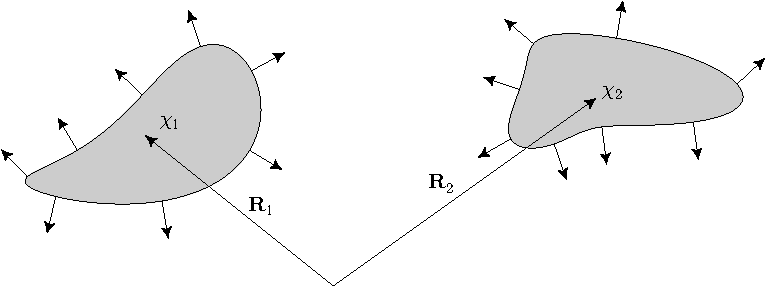
\includegraphics[width=\columnwidth]{fig/spud_sketch}
%   \caption{Geometry for interacting dielectric bodies of susceptibility $\chi_j$, centered at
%     $\vect{R}_j$ relative to the origin.  The surfaces mark $\sigma_j=0$, and the surface normal vectors $\hat{n}_j$
%     are also marked.}
%   \label{fig:spud_sketch}
% \end{figure}

\subsection{Pinning Paths to Surfaces}
\label{sec:path-pinning}
\subsubsection{Force}
The components of the force on a body can be found by differentiating the energy with respect to the center of that body.
For example, the force on body $2$, in direction $\hat{x}_i$ is 
found from the directional derivative of the spatial path integral~(\ref{eq:spatial_path_integral}) with respect to $R_{2,i}$,
\begin{align}
  F_{2,i}:=-\frac{\partial W}{\partial R_{2,i}}
  =-\alpha\int d\vect{x}_0 
  \biggdlangle \frac{\chi_2\hat{x}_{i}\cdot\langle \nabla\sigma_2\delta(\sigma_2)\rangle}
  {\langle\epsr\rangle^{\alpha+1}}\biggdrangle.
\end{align}
% where 
% \begin{equation}
%   \frac{\partial}{\partial R_{2,i}}\epsr = -\hat{R}_{2,i}\cdot\nabla\sigma_2(\vect{x}-\vect{R}_2)\delta(\sigma_2).
% \end{equation}
The force can be simplified by using the path-averaged $\delta$-function to 
restrict the paths to lie on the surface of the body.  For a generic ensemble-averaged path integral
integrated against a potential $\vect{g}[\vect{x}(t)]$, integrating out the $\delta$-function and 
simplifying the path-average yields
\begin{align}
  &\int d\vect{x}_0\bigdlangle \vect{g}[\vect{x}(t)]\!\cdot\!\langle \nabla\sigma_2\delta(\sigma_2)\rangle\bigdrangle\nonumber\\
  % &= \int d\vect{x}_0\bigdlangle \vect{g}(\vect{x})\!\cdot\!\langle \nabla\sigma_2\delta(\sigma_2)\rangle\bigdrangle \nonumber\\
  &\hspace{0.5cm}= \int \!\!d\vect{x}_0\biggdlangle \vect{g}[\vect{x}(t)]\!\cdot\!
  \frac{\nabla\sigma_2(\x0)}{|\nabla\sigma_2(\x0)|}\biggdrangle_{\sigma_2(\vect{x}_0-\vect{R}_2)=0},
  \label{eq:delta-normal}
\end{align}
where $\dlangle\cdots\drangle_{\sigma_2(\vect{x}_0-\vect{R}_2)=0}$ denotes the ensemble average over 
Brownian bridges subject to constraint on that $\vect{x}_0$ lie on the surface of body 2.
The renormalized force vector can be found by summing over all force components and subtracting off
the equivalent single-body expression,
\begin{align}
  \vect{F}_{2}&=
  -\alpha\!\! \int d\vect{x}_0  \chi_2\hat{n}_2(\vect{x}_0) \nonumber\\
  &\hspace{0.5cm}\times 
  \Biggdlangle\frac{1}{\langle\epsilon_{\mathrm{r},12}\rangle^{\alpha+1}}-\frac{1}{\langle\epsilon_{\mathrm{r},2}\rangle^{\alpha+1}}
  \Biggdrangle_{\sigma_2(\vect{x}_0-\vect{R}_2)=0},
  \label{eq:pinning_force}
\end{align}
where the unit surface normal vector for body 2 is defined as
\begin{equation}
  \hat{n}_2(\x0) := -\frac{\nabla \sigma_2(\x0-\vect{R}_2)}{|\nabla \sigma_2(\x0-\vect{R}_2)|}.
\end{equation}
The force on a body is found by starting the paths on the surface of that body,
and weighting the worldline contributions by the surface normal at the starting point.  
To compute the force it is still necessary to integrate over times $\cT$, with weight $\cT^{1+D/2}$.
Since different sections of the surface interact with the other body at different times $\cT$, each section's
contribution to the force will have differing weights, leading to an overall net force.

\subsubsection{Gradient of the Force}
This method can be easily extended to the second derivative of the worldline energy, which 
computes the potential curvature.  
\begin{equation}
  C_{ij} := \frac{\partial^2W}{\partial R_{2,i}\partial R_{2,j}}.
\end{equation}
For a dielectric describing two bodies, the derivatives with respect to $\vect{R}_2$ in direction $\hat{x}_i$, can be rewritten 
in terms of derivatives with respect to the first body's center $\vect{R}_1$, and the loop coordinates $\vect{x}_k$
\begin{align}
  \frac{\partial}{\partial R_{2,i}}\langle \epsr\rangle  
  =& \bigg(\sum_{k=1}^N\frac{\partial}{\partial {x}_{k,i}}-\frac{\partial}{\partial R_{1,i}}\bigg)\nonumber\\
  & \times[\langle \epsilon_1(\vect{x}-\vect{R}_1)\rangle+\langle\epsilon_2(\vect{x}-\vect{R}_2)\rangle],
  \label{eq:shift_derivative}
\end{align}
where $x_{k,i}$ is the $i^\text{th}$ component of the path position $\vect{x}_k$.  
The first derivative can be carried out as before,
\begin{align}
  C_{ij} = &      \alpha\int d\vect{x}_0 \biggdlangle 
  \hat{x}_{i}\cdot\bigg(\sum_k\frac{\partial}{\partial x_{k,i}}-\frac{\partial}{\partial R_{1,i}}\bigg)\nonumber\\
  &\hspace{3cm}\times\bigg[\chi_2
  \frac{\hat{x}_{j}\cdot\langle \nabla\sigma_2\delta(\sigma_2)\rangle}
  {\langle\epsr\rangle^{\alpha+1}}\bigg]\biggdrangle.
\end{align}
It is possible to integrate by parts so the derivatives with respect to the path positions $\vect{x}_k$, 
instead act on the Gaussian probability density,
 which yields a term proportional to $\sum_{k}(2\vect{x}_k-\vect{x}_{k+1}-\vect{x}_{k-1})$.
This sum of path increments vanishes for closed paths, and thus this term can be dropped.  
The remaining derivative can be straightforwardly evaluated,
and using Eq.~(\ref{eq:delta-normal}), there are now two path-averaged delta-functions which 
pin the paths to lie on different surfaces.  The first $\delta$-function pins the paths to start on
the first body, while the second $\delta$-function pins a different point of the path to lie on the second body,
and averages over which point is pinned.
The resulting expression for the potential curvature is 
\begin{align}
  C_{ij}&=
  \alpha(\alpha+1)\chi_1\chi_2\int d\vect{x}_0 \sum_{k=1}^{N-1}\frac{1}{N}
  \mathcal{G}(\vect{x}_0,\vect{x}_k,k)
  \nonumber\\
  &\hspace{0.5cm} \times\biggdlangle \frac{[\hat{x}_{i}\cdot\hat{n}_1(\vect{x}_0)][\hat{x}_{j}\cdot\hat{n}_2(\vect{x}_k)]}
  {\langle \epsilon_{\mathrm{r},12}\rangle^{\alpha+2}}     \biggdrangle_{\sigma_1(\vect{x}_0-\vect{R}_1)=0\atop \sigma_2(\vect{x}_k-\vect{R}_2)=0}.
  \label{eq:potential_curvature}
\end{align}
where 
\begin{equation}
  \mathcal{G}(\vect{x}_0,\vect{x}_k,k)=\frac{e^{-N(\vect{x}_0-\vect{x}_k)^2/(2 k(N-k)\Delta \cT)}}{(2\pi \Delta \cT)\sqrt{k (N-k)}}
\end{equation}
is the Gaussian normalization factor from fixing $\vect{x}_k$ after $k$ steps, and returning to $\vect{x}_0$
in $N-k$ steps.  There is no need for any further renormalization, since this expression is only non-zero in the presence 
of both bodies, and $\mathcal{G}$ exponentially cuts off terms at small $\cT$.    
\subsubsection{Torque}
The torque on a body can be found from the first order variation in the energy as that body is
infinitesimally rotated about some axis.  
For concreteness, consider perturbing the dielectric by rotating the second body about its center
by angle $\phi$ about axis $\hat{m}$,
% \begin{equation}
%   K_m = -\partial_\phi W,
% \end{equation}
%where the perturbed dielectric is 
\begin{equation}
  \epsr(\vect{x}) = 1+\chi_1\theta[\sigma_1(\vect{x}-\vect{R}_1)]
  +\chi_2\theta\big\{\sigma_2[\mathcal{R}(\phi)(\vect{x}-\vect{R}_2)]\big\}.
\end{equation}
The infinitesimal rotation matrix is given by 
\begin{equation}
  \mathcal{R}_{ij}(\phi) = \delta_{ij} - \phi m_k\epsilon_{ijk},
\end{equation}
where $\epsilon_{ijk}$ is the antisymmetric Levi-Civita tensor, and throughout this subsection
there are implicit sums over repeated indices.    
The torque path integral can be written as 
\begin{equation}
  K_m = \alpha\chi_2\int d\vect{x_0} \biggdlangle \frac{\langle \partial_\phi[\mathcal{R}_{ij}(\phi)(x_j-R_{2,j})]
    \partial_i \sigma_2\delta(\sigma_2)\rangle}{\langle \epsr\rangle^{\alpha+1}}\biggdrangle
\end{equation}
This can be simplied into a more intuitive form, by pinning the paths to start on the surface of the second body,
and using the form of the infinitesimal rotation to write the result as a cross-product 
via $(\vect{a}\wedge\vect{b})_i=\epsilon_{ijk}a_jb_k.$  
In this case the axis $\hat{m}$ is also arbitrary, and we can use $K_m=\hat{m}\cdot\vect{K}$ to 
sum over all components of the torque.  
The full torque worldline path integral is then 
\begin{align}
  \vect{K} =& \alpha\chi_2  \int d\vect{x}_0 
  \biggdlangle \big[(\vect{x}_0-\vect{R}_{2})\wedge \hat{n}_2(\vect{x}_0)\big]\nonumber\\
  &\hspace{0.5cm}\times \bigg[\frac{1}{\langle \epsilon_{\mathrm{r},12}\rangle^{\alpha+1}}
  -\frac{1}{\langle \epsilon_{\mathrm{r},2}\rangle^{\alpha+1}}\bigg]\biggdrangle_{\sigma_2(\vect{x}_0-\vect{R}_2)=0}.
\end{align}
This has the intuitive interpretation of finding the total torque on the body by 
integrating over its surface and taking the cross-product of the vector from the body's center to a surface
element with the force density at that surface element.  

\subsubsection{Casimir--Polder Force}

We briefly note that an alternative expression for the Casimir--Polder force on an atom near a surface
can be found in analogy to the potential curvature in Eq.~(\ref{eq:potential_curvature}).
The force on the atom is $F\subCP = -(\partial E\subCP)/(\partial x_{0,i})$.
  In Sec.~\ref{sec:partial_average} we took the derivatives of the path integral immediately,
  with the dominant contribution coming from the Gaussian probability distribution.  
  Instead, one can change the coordinates to $\vect{x}(t)=\vect{x}_0+\vect{y}(t)$, where 
  $\vect{y}(t)$ is a Brownian bridge starting and returning to the origin, $\vect{y}(0)=\vect{y}(\cT)=0$.
  The resulting force expression is
\begin{align}
  F_i =&\, -\frac{\hbar c\alpha_0}{4(2\pi)^{D/2}}\int \frac{d\cT}{\cT^{1+D/2}}\biggdlangle 
  \frac{\partial}{\partial x_{0,i}}\langle\epsr\rangle^{-3/2}
  \biggdrangle_{\vect{y}(t)},
\end{align}
where this path integral considers the change in energy as the whole path is translated,
while the results in Sec.~\ref{sec:partial_average}
correspond to shifting only the origin of the path, while keeping the rest of the path fixed.
The derivatives can be carried out, which for step-wise media create delta-functions.  In analogy 
with the potential curvature, since the starting point is fixed, one must still average over 
pinning other path points to lie on the dielectric surface.  
In which case after summing over all components the Casimir--Polder force is 
\begin{align}
  \vect{F}\subCP&=-\frac{3\hbar c\alpha_0}{8(2\pi)^{D/2}}
  \int_0^\infty \frac{d\cT}{\cT^{1+D/2}}
   \nonumber\\
   &\hspace{0.5cm} \times   \sum_{j}\sum_{k=1}^{N-1}\frac{\chi_j}{N}\mathcal{G}(\vect{x}_A,\vect{x}_k,k)
\biggdlangle \frac{\hat{n}_j(\vect{x}_k)}
  {\langle \epsilon_{\mathrm{r}}\rangle^{5/2}}     \biggdrangle_{\sigma_j(\vect{x}_k-\vect{R}_j)=0},
\end{align}
where we have reverted to using $\vect{x}(t)$ paths, 
and have restored the $\cT$-integral and constants for comparison with earlier results.

\subsection{Occupation Number}
\label{sec:occupation}

The preceding methods offer an intuitive picture of the Casimir force,
however they are poorly behaved as one takes the strong coupling limit.  
For a typical path of $N$ steps pinned to the surface, approximately half 
of the path will lie inside the body.  For $\chi\gg N$, the denominator $\langle\epsr\rangle^{-1/2}$ dominates
the integrand, so estimate of the derivatives tends to zero as $\chi^{-1/2}$ for almost all paths.  
Only rare paths which start on the surface, but do not enter the bulk of the body will contribute significantly.  
As a result the estimated force goes to zero in the strong-coupling limit.
In this section we develop an alternative expression which is better behaved in the strong-coupling
limit and makes direct contact with prior work on Dirichlet worldlines.  

In a similar fashion to Eq.~(\ref{eq:eps_gamma}), the spatial path integral can be written in exponential form via the Gamma function,
\begin{align}
  W &= \frac{1}{\Gamma[\alpha]}\int d\vect{x}_0 \int ds\, s^{\alpha-1}e^{-s}\nonumber\\
  &\hspace{0.5cm}\times\bigdlangle e^{-\langle \sum_r\chi_r\theta_r(\vect{x})\rangle} - e^{-\sum_r\chi_r\theta_r(\vect{x}_0)}\bigdrangle\label{eq:W_exp2}
\end{align}
where we have introduced a shorthand notation $\theta_r(\vect{x}) = \theta(\sigma_r[\vect{x}-\vect{R}_r])$.
% This exponential form is similar to the approach required to account for non-zero temperature and material
% dispersion~\cite{Mackrory2016}.  The exponential expression also places the integrand in a suitable form 
% to exploiting relevant Feynman-Kac formulae.  
The exponential path-integral for two bodies, after the single-body expressions have been factored out can 
be factorized as 
\begin{align}
  W &= \frac{1}{\Gamma[\alpha]}\int d\vect{x}_0 \int ds\, s^{\alpha-1}e^{-s}\nonumber\\
  &\hspace{0.5cm}\times\Bigdlangle 
  (e^{-\langle \chi_1\theta_1(\vect{x})\rangle}-1)(e^{-\langle \chi_2\theta_2(\vect{x})\rangle}-1)\nonumber\\
  &\hspace{1.25cm}
  -(e^{- \chi_1\theta_1(\vect{x}_0)}-1)(e^{-\chi_2\theta_2(\vect{x}_0)}-1)\Bigdrangle\label{eq:W_exp2}
\end{align}
\comment{Pretty sure a Gies paper does a similar factorization.}
%\begin{align}
  % &e^{-s}[1+e^{-s\langle \chi_1(\vect{x})+\chi_2(\vect{x})\rangle } 
  % - e^{-s\langle \chi_1(\vect{x})\rangle }-e^{-s\langle \chi_2(\vect{x})\rangle}]\nonumber\\

The exponential of the path-averaged potential can be written as a product of potentials 
for each increment, and the potential can be simplified for step-function dielectrics,
\begin{align}
  e^{-s \langle\chi_r\theta_r(\vect{x})\rangle}= \prod_{k=0}^{N-1}
  \left[\bar{\theta}_{r,k}+\theta_{r,k}e^{-s\chi_r/N}\right].
\end{align}
where we introduced $\theta_{r,k} := \theta[\sigma_r(\vect{x}_k-\vect{R}_r)],$ 
and $\bar{\theta}_{r,k}:=1-\theta_{r,k}$.  The force path integral can be computed by differentiating
Eq.~(\ref{eq:W_exp2}) with respect to the body position $\vect{R}_2$,
% \begin{equation}
%   F_2 = (-1)\alpha\int d\vect{x}_0\int ds\,s^{\alpha-1}e^{-s}\dlangle (1-\mathcal{V}_1)\mathcal{W}_2\drangle,
% \end{equation}
% where 
% \begin{align}
%   \mathcal{W}_r &:= \big(e^{-s\chi_r/N}-1\big)\sum_j\hat{n}_2(\vect{x}_j)\delta_{r,j}\nonumber\\
%   &\hspace{0.5cm} \times\prod_{k\ne j}\left\{1+\theta_{r,k}\big(e^{-s\chi_r/N}-1\big)\right\},
% \end{align}
% where $\delta_{r,j}$ restricts $\sigma_r(\vect{x}_j-\vect{R}_r)=0$.  
% Full force version with explicit steps. 
\begin{align}
  \vect{F}_2 =& -\frac{1}{\Gamma[\alpha]}\int d\vect{x}_0\int ds\,s^{\alpha-1}e^{-s}\biggdlangle 
  \big(e^{-s\chi_2/N}-1\big)\nonumber\\
  &\times\sum_{j=0}^{N-1}\vect{n}_2(\vect{x}_j)\delta_{2,j}
  \prod_{k\ne j}\left(\bar\theta_{2,k}+\theta_{2,k}e^{-s\chi_2/N}\right)\nonumber\\
  &\times\bigg[1-\prod_{n}\left(\bar{\theta}_{1,n}+\theta_{1,n}e^{-s\chi_1/N}\right)\bigg]\biggdrangle,
\end{align}
where we have introduced $\delta_{r,j} = \delta[\sigma_r(\vect{x}_j-\vect{R}_r)]$.
The $s$ integral can be carried out if the integrand is rearranged into terms with 
a definite number of points inside each body.  
We define the indicator functions
\begin{equation}
  \I[r]n:= \sum_{j_1=1}\sum_{j_2>j_1}\cdots\sum_{j_{n}>j_{n-1}}\theta_{r,j_1}\theta_{r,j_2}\cdots\theta_{r,j_n},
\end{equation}
where the subscripts $n$ counts the number of points of the path that are inside body $r$,
and all of the sums terminate at $N$.  There are further restrictions on which of these 
terms contribute.  Due to the presence of the $\delta$-functions, only $N-1$ points are free to 
enter the bodies.  This further implies that the number of points inside both bodies must be less than $N-1$. 
Finally, due to the renormalization only paths with at least one point inside body 1 contribute.  
The re-arranged force is 
% \begin{align}
%   \vect{F}_2 =& -\frac{1}{\Gamma[\alpha]}\int d\vect{x}_0\int ds\,s^{\alpha-1}e^{-s}\biggdlangle 
%   \big(e^{-s\chi_2/N}-1\big)\nonumber\\
%   &\times\sum_{j=0}^{N-1}\vect{n}_2(\vect{x}_j)\delta_{r,j}\sum_{n=0}^{N-1}e^{-sn\chi_2/N} \I^{(2)}_{n}\nonumber\\
%   & \bigg(1-\sum_{m=0}^{N-n-1} e^{-s m \chi_1/N} \mathbf{I}^{(1)}_{m}\bigg)
%   \biggdrangle,
% \end{align}
% Restrict sums since one point is fixed to line on body, so $N-1$ points free.  If $n$ points inside
% one body, at most $N-1-n$ points in second body.  
% Rearranging, and noting only $m>0$ contributes after renormalization.  
% Can also write $1 = \sum_{m=0}^N \mathbf{I}_{m,r}$.
\begin{align}
  \vect{F}_2 =& (-1)\int d\vect{x}_0\int ds\,s^{\alpha-1}e^{-s}\biggdlangle \sum_{j=0}^{N-1}\hat{n}_2(\vect{x}_j)\delta_{r,j}\nonumber\\
  &\times\sum_{n=0}^{N-1}\I[2]n
  \big(e^{-s(n+1)\chi_2/N}-e^{-sn\chi_2/N}\big)\nonumber\\
  &\times \sum_{m=1}^{N-n-1}\big(1- e^{-s m \chi_1/N} \big)\I[1]m
  \biggdrangle,
\end{align}
The $s$ integral can be straightforwardly carried out term by term, and the $\delta$-function
can be used to pin paths onto the surface, with the result
\begin{align}
  \vect{F}_2 =& (-1)\int d\vect{x}_0 \sum_{j=0}^{N-1}\sum_{n=0}^{N-1}\sum_{m=1}^{N-n-1}\nonumber\\
  &\hspace{0.5cm}\times \bigdlangle\hat{n}_2(\vect{x}_j)
  \I[1]m\I[2]n f_{m,n}\bigdrangle_{\sigma_2(\vect{x}_j-\vect{R}_2)=0}
  \label{eq:occupation_force}
\end{align}
where 
\begin{align}
  f_{m,n}&:=c_{m,n}-c_{m,n+1}-c_{0,n}+c_{0,n+1}\\
  c_{m,n} &:= \bigg( 1 + \frac{m\chi_1+n\chi_2}{N}\bigg)^{-\alpha}.
\end{align}
% \begin{align}
%   f_{n,m}=& \frac{[1+(m\chi_1+n\chi_2)/N]^{-\alpha} -[1+n\chi_2/N]^{-\alpha}\nonumber\\
%   &\hspace{0.5cm}-\big\{1+[m\chi_1+(n+1)\chi_2]/N\big\}^\alpha \nonumber\\
%   &\hspace{0.5cm}+[1+(n+1)\chi_2/N]^{-\alpha}.
% \end{align}
In this result the indicator functions carry the position dependence, while $f_{n,m}$ carries
the dependence on material properties based on the number of points inside each body.  
This expression is well-behaved in the $\chi\rightarrow\infty$ limit, where only 
the $n=0, m>0$ terms contribute.  In the strong-coupling limit, the main contribution to the 
force comes from paths that just graze the second surface, while also entering the first body.  

This is exactly the construction of paths employed by Gies and Weber for computing 
forces in the sphere-plate and cylinder-plate geometries in the Dirichlet limit~\cite{Weber2010}.  
In that work they shift the paths so that the path just grazes the plane.  The force on the planar
surface is computed by integrating the over the times when the path intersects the spherical or cylindrical surface.
The expressions presented here extend their results by accounting for finite $\chi$, 
and are framed in terms of general geometries.  

In general, different classes of paths are important in the finite $\chi$ and strong-coupling 
cases.  At small $\chi$, the most important path statistic is the sojourn time within the bodies,
while in strong-coupling regime, the first-touching time is the most important statistic.    
This is correspondence was previously used to describe the numerical convergence properties of as 
the resolution of the paths was varied~\cite{Mackrory2016}.  
More practically, this makes it difficult to use a single class of loops to evaluate the potential at all $\chi$:
in weak-coupling one wants a path-ensemble that enters all of the bodies, while in strong-coupling
it is the paths that just touch the surfaces that are most important.

The expressions for the force in Eqs.~(\ref{eq:pinning_force}) and (\ref{eq:occupation_force})
reflect taking two limits in different orders, namely the taking the large $N$ limit and differentiation.  
The first derivation assumed an arbitrarily fine path where $N\gg \chi$ for all $\chi$.  Under
differentiation the arbitrarily fine paths can be pinned to the surface, and there is a range of 
$\cT$ where the integrand is non-zero.  However for a discrete path of length $N$, for sufficiently large $\chi$, 
this range of $\cT$ is inaccessible, and thus the naive numerical estimate fails.    
The second derivation instead takes the $N\rightarrow\infty$ expression last, while using well-behaved
expressions as $\chi\rightarrow\infty$, as is better suited to a numerical method based on discrete paths.  
This method instead highlights finding the times when the number of points inside each body 
change.  

% Energy
% \begin{equation}
%   W = \int d\vect{x}_0 \sum_{n+m \le N}\dlangle \mathbf{I}_{n,m}[\vect{x}(t)] w_{n,m}\drangle 
% \end{equation}
% where 
% \begin{align}
%   w_{n,m} =& 1+\frac{1}{[1+(n\chi_1+m\chi_2)/N]^\alpha}\nonumber\\
%   &\hspace{0.5cm}-\frac{1}{(1+n\chi_1/N)^\alpha}-\frac{1}{(1+m\chi_2/N)^\alpha}
% \end{align}
% Note that all of the position dependence is in the indicator function, which serves 
% as a shorthand for the various combinatorics of step-functions.    

For completeness we note the analogous expressions for the torque and potential curvature.  
The torque path integral is 
\begin{align}
  \vect{K}_2 =& (-1)\int d\vect{x}_0 \sum_{j=0}^{N-1}\sum_{n=0}^{N-1}\sum_{m=1}^{N-n-1}\nonumber\\
  &\hspace{0.5cm}\times \bigdlangle(\vect{x}-\vect{R}_2)\wedge\hat{n}_2(\vect{x}_j)
  \mathbf{I}_{m,1}\mathbf{I}_{n,2}f_{n,m}\bigdrangle_{\sigma_2(\vect{x}_j-\vect{R}_2)=0}.
\end{align}
% Potential curvature
% \begin{align}
%   C_{ij} =& \int d\vect{x}_0\int ds\, s^{\alpha-1}e^{-s}\nonumber\\
%   &\biggdlangle\big(e^{-s\chi_1/N}-1\big)\big(e^{-s\chi_2/N}-1\big)\nonumber\\
%   &\times\sum_{j}\hat{n}_1(\vect{x}_j)\delta_{1,j}\prod_{r\ne j}\left[\bar\theta_{1,k}+\theta_{1,k}e^{-s\chi_1/N}\right]\nonumber\\
%   &\times\sum_{k}\hat{n}_2(\vect{x}_k)\delta_{2,k}\prod_{s\ne k}\left[\bar\theta_{2,k}+\theta_{2,k}e^{-s\chi_2/N}\right]
%   \biggdrangle
% \end{align}
% Group via indicator function.  
% \begin{align}
%   C_{ij} =& \frac{1}{\Gamma}\int d\vect{x}_0\int ds\, s^{\alpha-1}e^{-s}\big(e^{-s\chi_1/N}-1\big)\big(e^{-s\chi_2/N}-1\big)\nonumber\\
%   &\biggdlangle
%   \sum_{j,k}\vect{n}_1(\vect{x}_j)\vect{n}_2(\vect{x}_k)\delta_{1,j}\delta_{2,k}\nonumber\\
%   &\times\sum_{n=0}^{N-2}\sum_{m=0}^{N-n-2}\I[1]n\I[2]m e^{-s(m\chi_1+n\chi_2)/N}
%   \biggdrangle
% \end{align}
% Only $n=m=0$ contributes in strong-coupling limits.  
and the potential curvature is given by
\begin{align}
  C_{ij} =& \int d\vect{x}_0\biggdlangle 
  \sum_{j,k=0}^{N-1}\hat{n}_1(\vect{x}_j)\hat{n}_2(\vect{x}_k)\mathcal{G}(\vect{x}_j,\vect{x}_k,k-j)
  \nonumber\\
  &\hspace{1cm} \times\sum_{n=0}^{N-2}\sum_{m=0}^{N-n-2}\I[1]n\I[2]m g_{m,n}
  \biggdrangle_{\sigma_1(\vect{x}_j-\vect{R}_1)=0\atop \sigma_2(\vect{x}_k-\vect{R}_2)=0}
\end{align}
where 
\begin{align}
  g_{m,n}=c_{m+1,n+1}+c_{m,n}-c_{m+1,n}-c_{m,n+1}
  % c_{n,m}&=\bigg(1+\frac{m+1}{N}\chi_1+\frac{n+1}{N}\chi_2\bigg)^{-\alpha}+\bigg(1+\frac{m}{N}\chi_1+\frac{n}{N}\chi_2\bigg)^{-\alpha}\nonumber\\
  % &-\bigg(1+\frac{m+1}{N}\chi_1+\frac{n}{N}\chi_2\bigg)^{-\alpha}-\bigg(1+\frac{m}{N}\chi_1+\frac{n+1}{N}\chi_2\bigg)^{-\alpha}
  % c_{n,m}&=\{1+[(m+1)\chi_1+(n+1)\chi_2]/N\}^{-\alpha} + [1+(m\chi_1+n\chi_2)/N]^{-\alpha}\nonumber\\
  % &-\{1+[(m+1)\chi_1+n\chi_2]/N\}^{-\alpha}-\{1+[m\chi_1+(n+1)\chi_2]/N\}^{-\alpha}
\end{align}
In the strong-coupling limit, the potential curvature is dominated by terms with $n=m=0$,
which correspond to paths that graze both bodies, while not entering either body.  

\subsubsection{Numerical Implementation}

The path integral for the potential curvature in the occupation numbers apporach requires paths 
that are constrained by $\sigma_1(\vect{x}_j)$ and $\sigma_2(\vect{x}_k)$.  
There are a couple approaches to take here.  First, we could generate paths and then retroactively
find points close to the requisite surfaces, and perturb those paths such that the points do touch the 
surface.  We would then sum over all possible combinations of the indices close to the surfaces.
In this approach we would sample a position $x_0$, and then a time $\cT$.  Then we would find the 
near-intersections, and sum the integral over perturbing these.  

Alternatively,  we can enforce the touching constraint directly and make the paths touch the bodies by constructing
paths which are fixed at steps $j$ and $k$ to touch the surface, and sum over all $j,k\in {1,N}$.  
Evidently the direct approach will create many paths with small contributions, particular if $j-k \sim 1$.
This can be made more efficient by exploiting the Gaussian factor as a probability distribution.

In computing the energy the Gaussian is introduced for the purpose of importance sampling, and must
be factored out.
In this case, it is already manifest, and should be taken into account.  
We would sample times from Eq.~\ref{eq:exp_T}, with 
\begin{equation}
  T_0 = \frac{N^2d^2}{2k(N-k)}
\end{equation}
where $k$ is the difference in indices at the crossing points.
The result of using this is as our probability distribution is to factour out a normalization constant,
which leaves the integrand as 
\begin{equation}
  c=\left(\frac{N^2d^2}{2k(N-k)}\right)^{-m+1}\frac{N}{2\pi \sqrt{k(N-k)}}
    =\frac{2^{m-1}}{2\pi d^{2m-2}} [\frac{k(N-k)}{N^2}]^{m-3/2}
\end{equation}
where $m=1+D/2+1$, accounting for the path integral normalization and the Gaussian factors of $T$.  

The $k$ values can be sampled via a lookup table.  For moderate $N$, this will be easily computed
once for each process.  

\section{Results}
    \subsection{Atom-Plates}
    
    \subsubsection{TE Polarization}
    \begin{enumerate}
      \item Simple Trapezoidal rule
      \item Convergence arguments
      \item ``Exact methods''
    \end{enumerate}
    
    \subsubsection{TM Polarization}

    \begin{enumerate}
      \item Need gradient estimation.  Use Malliavin calculus~\cite{Fournie1999, Chen2007,Kohatsu-Higa2003}.
        Formal introductions \cite{Nualart2006, Malliavin2006, DiNunno2009}.
      \item Gradients required for computing forces.  
      \item Birth-death methods to handle product of increments.  Related to Genealogical 
        methods used in rare-event simulation.  
      \item Histogram of raw values, with/without birth-death.
      \item 
    \end{enumerate}
    
    % \section{Planar Dielectrics}




    % \section{Atom-Sphere}
    % \section{Atom-Cylinder}

    % \section{Plane-Sphere}

%%% Local Variables: 
%%% mode: latex
%%% TeX-master: "thesis_master"
%%% End: 
